%% ---------------------------------------------------------------------------
\section{Results}\label{sec:results}

All numbers in this section are produced by the released scripts. Unless stated otherwise, errors are medians over the frames of a test set (600 frames for ID, OOD-G and OOD-L, 300 for DES), the proposed surrogate is the five-network ensemble with variance-weighted projection, and single numbers refer to the first of five independent training runs (ensemble 0); the variation over the five runs is reported in Section~\ref{sec:stats}.

\begin{figure}[p]
\centering
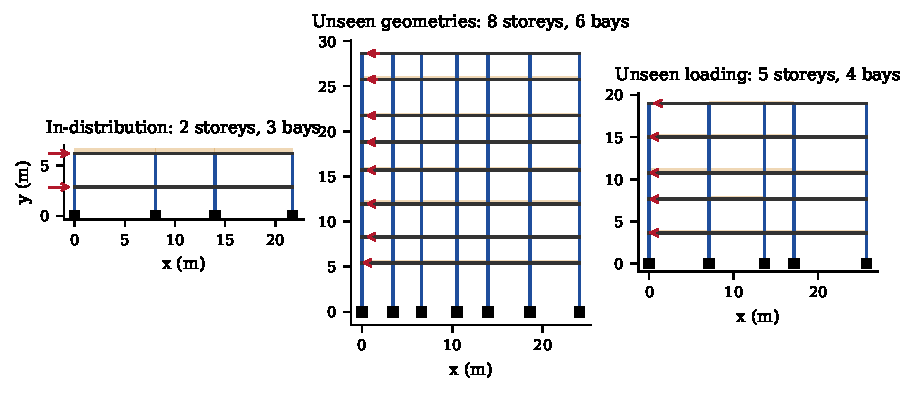
\includegraphics[width=\textwidth]{fig_frames.pdf}
\caption{Example frames from the four test sets. Blue: columns; black: beams; shaded: gravity line loads (scaled); red arrows: lateral floor forces; squares and triangles: fixed and pinned bases.}\label{fig:frames}
\end{figure}

\subsection{Dataset}
The 5{,}000-frame pool contains frames with 3 to 45 members (18 on average), the OOD-G set frames with 11 to 104 members (56 on average) and the DES set frames with 3 to 45 members (18 on average); Fig.~\ref{fig:frames} shows one frame of each set. A PyNite analysis of one frame (both load cases, including model construction and result extraction) took 37.5\,ms on average for the ID frames and 104.7\,ms for the larger OOD-G frames (Section~\ref{sec:cost}). Because sections and loads of the ID, OOD-G and OOD-L frames are sampled independently and are not sized for serviceability, the median largest inter-storey drift ratio is 0.46\% (ID) and 0.79\% (OOD-G), and 15\% and 25\% of these frames exceed 2\%. The design-driven frames are stiffer, with a median largest drift ratio of 0.18\%; 29\% of them exceed $h/400$ because the column sizing uses a simplified shear-building estimate. Since all models predict dimensionless responses that are exactly invariant to the load intensities and to $E$ (Section~\ref{sec:scaling}), the relative errors reported below do not depend on the load magnitudes.

\subsection{Accuracy on seen and unseen frames}\label{sec:accuracy}

\begin{table}[p]
\centering
\caption{Prediction errors on the in-distribution and design-driven test sets (medians over the frames, in \%, except the 95th percentile (p95) of $e_M$; last column: median relative nodal out-of-balance force). Bold: best value per column and set. The last row of each block gives the proposed surrogate as mean $\pm$ standard deviation of the per-run values over five independent training runs.}\label{tab:main}
\footnotesize
\setlength{\tabcolsep}{4pt}
\begin{adjustbox}{max width=\textwidth}
\begin{tabular}{lrrrrrr}
\toprule
Model & $e_{u_x}$ & $e_\mathrm{drift}$ & $e_M$ & $e_M$ (p95) & $e_N$ & Out-of-balance \\
\midrule
\inputtable{tables/tab_main_a.tex}
\bottomrule
\end{tabular}
\end{adjustbox}
\end{table}

\begin{table}[p]
\centering
\caption{As Table~\ref{tab:main}, for the unseen-geometry and unseen-loading test sets.}\label{tab:mainood}
\footnotesize
\setlength{\tabcolsep}{4pt}
\begin{adjustbox}{max width=\textwidth}
\begin{tabular}{lrrrrrr}
\toprule
Model & $e_{u_x}$ & $e_\mathrm{drift}$ & $e_M$ & $e_M$ (p95) & $e_N$ & Out-of-balance \\
\midrule
\inputtable{tables/tab_main_b.tex}
\bottomrule
\end{tabular}
\end{adjustbox}
\end{table}

Tables~\ref{tab:main} and~\ref{tab:mainood} compare the proposed surrogate with the five tabular baselines, and Fig.~\ref{fig:cdf} shows the full error distributions. On the in-distribution test set the proposed surrogate reaches median errors of 4.5\% for the horizontal displacement field, 4.9\% for the governing drift ratio, 2.4\% for the end-moment field and 0.6\% for the axial forces. The best baseline, gradient boosting, has 29.0\%, 30.2\%, 10.0\% and 3.2\%, so the graph surrogate is about four times more accurate for the member forces and six times more accurate for the displacements, although the baselines receive the same mechanics-informed features, targets and boundary conditions. The gap is largest for displacements, which depend on the stiffness of the whole frame and not only on local quantities. The design-driven frames, whose parameter correlations were never seen in training, are predicted as accurately as the ID frames: median errors of 4.4\% ($u_x$), 3.0\% (drift) and 2.0\% (moments), with a 95th percentile of the moment error of only 3.4\%, against 8.7\% (moments) and 37\% ($u_x$) for the best baselines.

\begin{figure}[p]
\centering
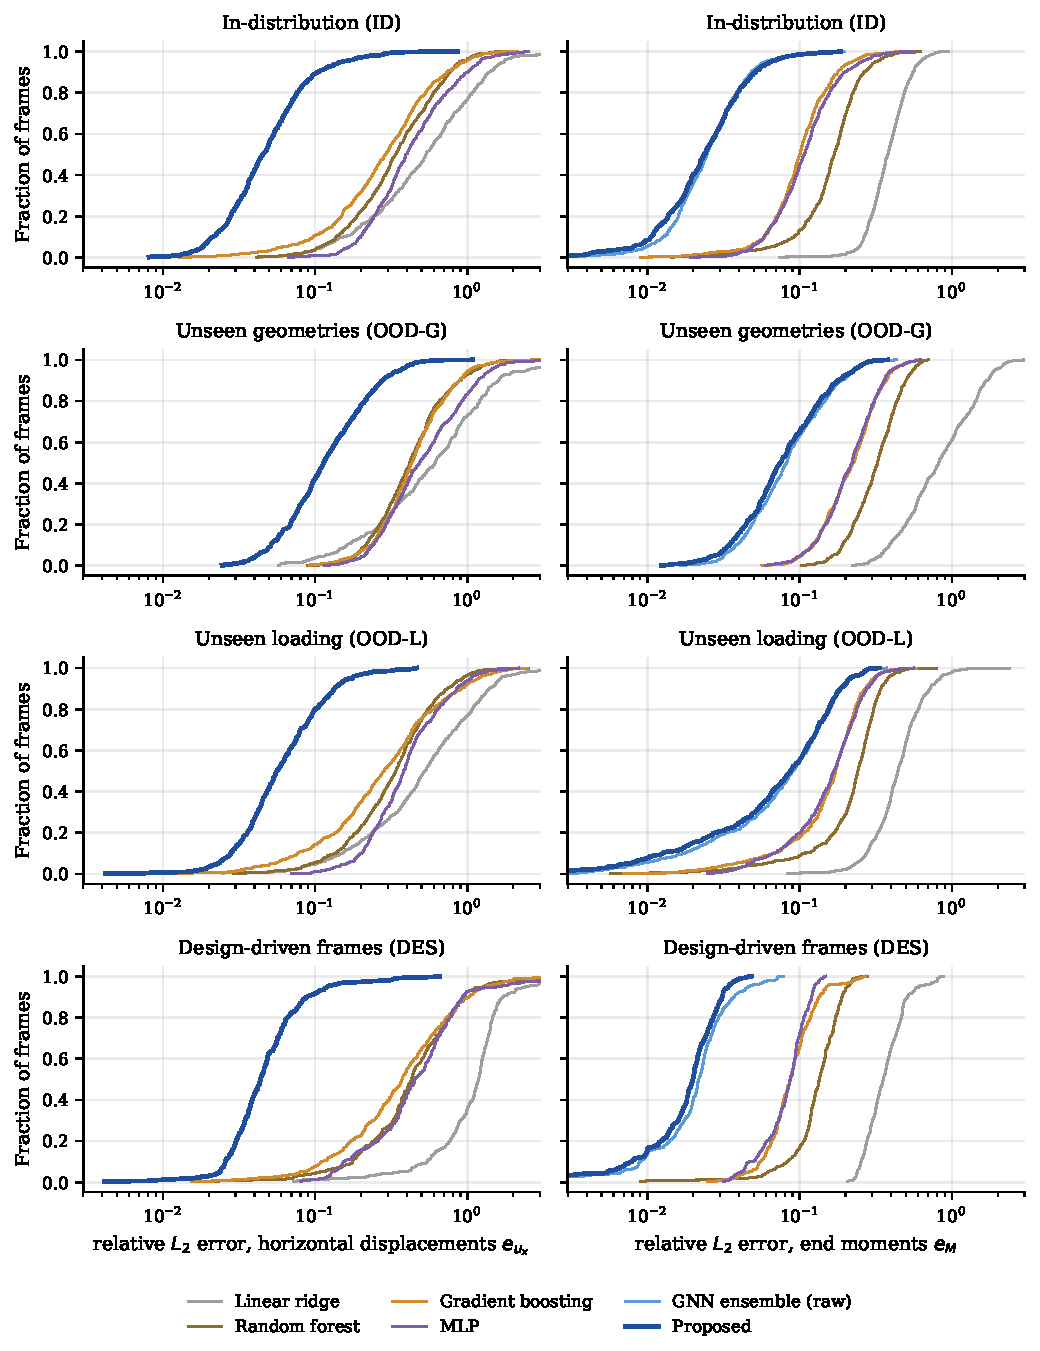
\includegraphics[width=\textwidth]{fig_error_cdf.pdf}
\caption{Cumulative distributions of the per-frame relative errors of the horizontal displacement field (left) and of the end-moment field (right) for the four test sets.}\label{fig:cdf}
\end{figure}

All models lose accuracy on the unseen geometries and load patterns, but the ranking is unchanged. For unseen geometries (up to eight storeys and six bays, against at most five and four in training) the proposed surrogate has a median moment error of 7.5\% and a median displacement error of 11.4\%, against 22.5\% and 43.1\% for gradient boosting; the governing-drift error is 13.7\%, whereas the tabular baselines have errors of 72--143\%. For unseen load patterns the median moment error is 8.7\% (gradient boosting 17.3\%, MLP 16.8\%) and the displacement error 5.6\%. The tails are heavy: the 95th percentile of the moment error is 22.6\% for unseen geometries and 21.4\% for unseen loading, which is not acceptable for design without further checks and motivates the referral rule of Section~\ref{sec:uqresults}. Figure~\ref{fig:parity} shows parity plots for the roof displacement and the largest end moment, and Fig.~\ref{fig:example} the end moments of a typical unseen-geometry frame.

\begin{table}[t]
\centering
\caption{Extended response metrics of the proposed surrogate: median and 95th percentile (p95) of the per-frame errors (\%), mean $\pm$ standard deviation over five independent training runs. Governing member: share of frames in which the member with the largest end moment is predicted as the largest (top-1) or among the three largest (top-3).}\label{tab:extended}
\footnotesize
\setlength{\tabcolsep}{3pt}
\begin{adjustbox}{max width=\textwidth}
\begin{tabular}{lrrrrrrrr}
\toprule
& \multicolumn{2}{c}{ID} & \multicolumn{2}{c}{OOD-G} & \multicolumn{2}{c}{OOD-L} & \multicolumn{2}{c}{DES}\\
\cmidrule(lr){2-3}\cmidrule(lr){4-5}\cmidrule(lr){6-7}\cmidrule(lr){8-9}
Metric & median & p95 & median & p95 & median & p95 & median & p95\\
\midrule
\inputtable{tables/tab_extended.tex}
\bottomrule
\end{tabular}
\end{adjustbox}
\end{table}

Table~\ref{tab:extended} extends the evaluation to the quantities an engineer checks. Vertical displacements and rotations are predicted with median errors of 3.2\% and 4.2\% on ID frames. The largest beam mid-span deflection, the largest end moment and the largest axial force, which govern serviceability and member design, are within 0.6\%, 0.8\% and 0.2\% of PyNite at the median, and the support reactions within 0.6\%; the 95th percentiles of these peak quantities stay below 4.5\% on the ID and DES sets. End shears follow the moments (median 1.2\%). The member with the largest end moment is identified correctly in about 94\% of the ID frames and is among the three predicted largest in almost all frames. On the unseen sets the peak quantities degrade much less than the full fields (largest moment 2.2\% and 2.5\% at the median for OOD-G and OOD-L), whereas the rotations and the governing drift ratio show the largest tails (95th percentiles of 28--40\% for the rotations and up to 97\% for the governing drift on OOD-G), so serviceability checks on unseen frames are the least reliable use of the surrogate.

\begin{figure}[p]
\centering
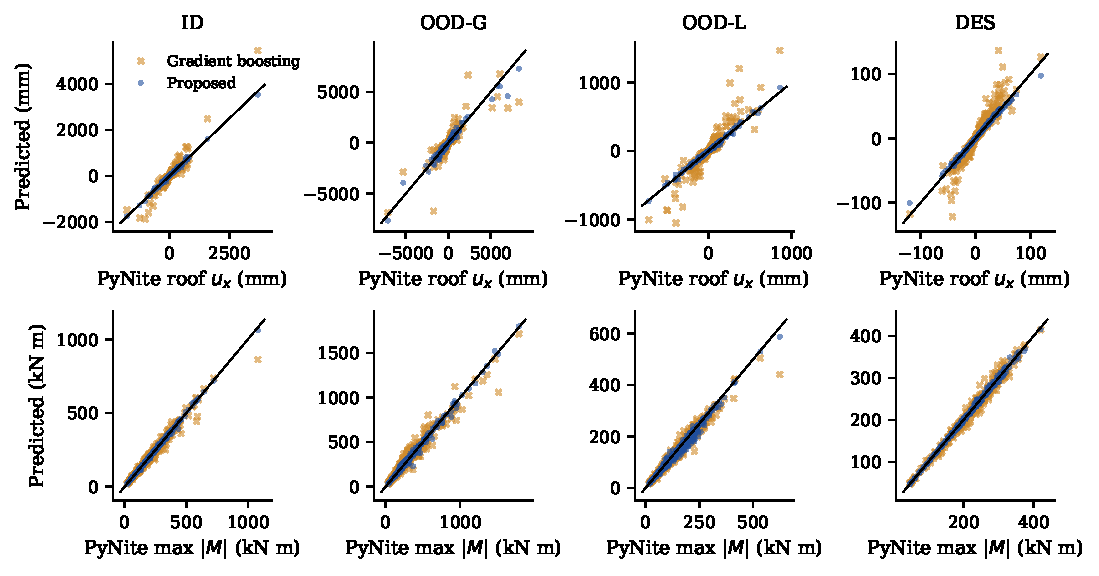
\includegraphics[width=\textwidth]{fig_parity.pdf}
\caption{Predicted versus PyNite roof displacement (top; mean of the roof nodes) and largest absolute end moment (bottom) for the proposed surrogate and the best tabular baseline.}\label{fig:parity}
\end{figure}

\begin{figure}[t]
\centering
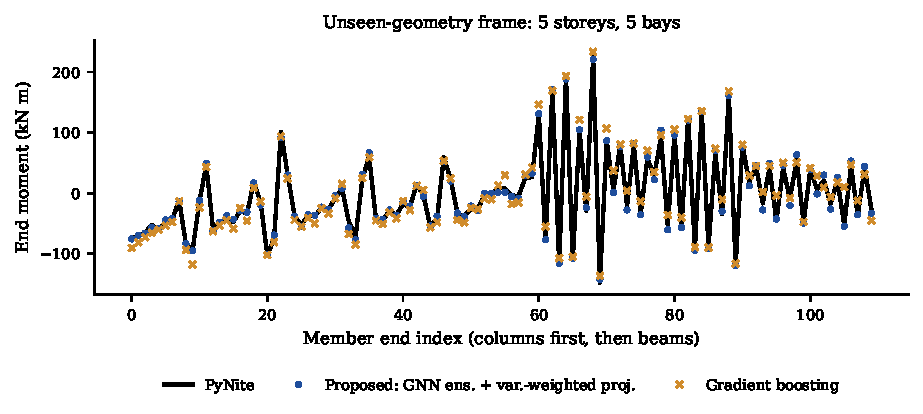
\includegraphics[width=\textwidth]{fig_example.pdf}
\caption{End moments of all members of an unseen-geometry frame (the OOD-G frame with the median number of members): PyNite, proposed surrogate and gradient boosting.}\label{fig:example}
\end{figure}

\subsection{Statistical robustness}\label{sec:stats}

\begin{table}[t]
\centering
\caption{Uncertainty of the headline results (moment error $e_M$, \%). Bootstrap: 95\% percentile-bootstrap interval over test frames for ensemble 0 (2{,}000 resamples). Across runs: mean and 95\% $t$-interval of the per-run median over five independent ensembles. Raw $-$ projected: reduction of the median $e_M$ by the variance-weighted projection, paired bootstrap for ensemble 0 and $t$-interval over the five runs.}\label{tab:stats}
\footnotesize
\begin{adjustbox}{max width=\textwidth}
\begin{tabular}{lccccc}
\toprule
Set & Median (bootstrap) & p95 (bootstrap) & Median (across runs) & Raw $-$ proj.\ (bootstrap) & Raw $-$ proj.\ (across runs)\\
\midrule
\inputtable{tables/tab_stats.tex}
\bottomrule
\end{tabular}
\end{adjustbox}
\end{table}

The five independent training runs (25 networks) give almost the same errors (Tables~\ref{tab:main}--\ref{tab:stats}): the per-run median moment error is $2.37\pm0.03\%$ (ID), $7.65\pm0.24\%$ (OOD-G), $8.79\pm0.32\%$ (OOD-L) and $1.99\pm0.08\%$ (DES), and the median displacement error $4.45\pm0.15\%$, $12.1\pm0.5\%$, $5.85\pm0.15\%$ and $4.45\pm0.12\%$. The variation between runs is much smaller than the sampling uncertainty of a single run over the test frames: the 95\% bootstrap interval of the ID median moment error of ensemble 0 is [2.24, 2.52]\%, and that of the 95th percentile [5.8, 7.2]\%. Every difference between the proposed surrogate and the tabular baselines in Tables~\ref{tab:main}--\ref{tab:mainood} is far larger than these intervals.

The effect of the projection on the median moment error is small and must be read with its intervals. On the ID set it lowers the median by 0.10 percentage points (2.46\%$\to$2.36\% for ensemble 0). The reduction has the same sign in all five runs (95\% $t$-interval [0.05, 0.14] points), but the paired bootstrap interval for a single run, [$-0.01$, 0.20] points, includes zero. The reduction is larger and significant in both senses on unseen geometries (0.53 points across runs, [0.33, 0.72]) and on the DES set (0.17, [0.08, 0.26]); on unseen load patterns the across-run interval includes zero. The projection should therefore be credited with exact equilibrium and a large reduction of the axial-force errors (Section~\ref{sec:eqresults}), and with a modest, consistent reduction of the moment errors, not with a decisive gain in moment accuracy.

\subsection{Graph-learning baselines, ablations and message-passing depth}\label{sec:graphbaselines}\label{sec:ablation}

\begin{table}[p]
\centering
\caption{Single graph networks (no ensembling, no projection): median $e_{u_x}$ and $e_M$ (\%), mean $\pm$ standard deviation over three training seeds. All models are trained on the same 3{,}000 frames for 150 epochs.}\label{tab:graph}
\footnotesize
\setlength{\tabcolsep}{3pt}
\begin{adjustbox}{max width=\textwidth}
\begin{tabular}{lrrrrrrrr}
\toprule
& \multicolumn{2}{c}{ID} & \multicolumn{2}{c}{OOD-G} & \multicolumn{2}{c}{OOD-L} & \multicolumn{2}{c}{DES}\\
\cmidrule(lr){2-3}\cmidrule(lr){4-5}\cmidrule(lr){6-7}\cmidrule(lr){8-9}
Model & $e_{u_x}$ & $e_M$ & $e_{u_x}$ & $e_M$ & $e_{u_x}$ & $e_M$ & $e_{u_x}$ & $e_M$\\
\midrule
\inputtable{tables/tab_graph.tex}
\bottomrule
\end{tabular}
\end{adjustbox}
\end{table}

\begin{table}[t]
\centering
\caption{Equilibrium and compatibility of the graph baselines (single networks, mean of three seeds): median relative out-of-balance force of the raw forces, median $e_M$ (\%) after Euclidean projection of the forces, median moment compatibility residual $r_{\mathrm{compat},M}$ (\%), and training time of one network on one CPU thread (min).}\label{tab:grapheq}
\footnotesize
\setlength{\tabcolsep}{3pt}
\begin{adjustbox}{max width=\textwidth}
\begin{tabular}{lrrrrrrr}
\toprule
& \multicolumn{3}{c}{ID} & \multicolumn{3}{c}{OOD-G} & \\
\cmidrule(lr){2-4}\cmidrule(lr){5-7}
Model & Eq.\ res. & $e_M$ proj. & $r_{\mathrm{compat},M}$ & Eq.\ res. & $e_M$ proj. & $r_{\mathrm{compat},M}$ & Train (min)\\
\midrule
\inputtable{tables/tab_graph_eq.tex}
\bottomrule
\end{tabular}
\end{adjustbox}
\end{table}

Table~\ref{tab:graph} compares single networks, so that the architecture is separated from the ensemble and the projection. Four findings stand out.

\emph{Mechanics-informed inputs and the load-case split matter more than the architecture.} The conventional GNN with physical inputs and targets has more than twice the displacement error of the proposed network on ID frames (14.3\% against 6.7\%) and 2.4--3.9 times on the unseen and design-driven sets, and 1.5 times the moment error on ID and OOD-G frames, although its moment error on unseen load patterns is lower (8.4\% against 10.0\%). Replacing the load-case split by a single combined load scale roughly doubles the displacement errors (12.5\% ID, 26.0\% OOD-G, 34.9\% DES) and raises the moment errors by up to 3.5 points (OOD-L unchanged), confirming the scaling argument of Section~\ref{sec:scaling}: in the combined case the lateral sway is masked by the much larger gravity scale.

\emph{The StructGNN-style network is a strong competitor.} With the same inputs and targets it reaches displacement errors similar to or lower than the proposed network (6.3\% ID, 12.3\% OOD-G, 7.1\% OOD-L) and slightly higher moment errors on ID, OOD-G and DES frames (4.2\%, 11.9\% and 3.9\% against 3.7\%, 11.3\% and 3.3\%); on unseen load patterns it is marginally better (9.7\% against 10.0\%). Its storey pseudo nodes and height-dependent depth carry global information quickly, which helps the displacements, at seven times the training cost (77 against 11 minutes per network on one thread). The proposed network with global pooling or with 16 message-passing steps gains in the same way (OOD-G displacement error 11.1\% and 11.8\% against 14.1\%) at little or no cost in moment accuracy. The accuracy of a single network is therefore not what distinguishes the proposed framework; the distinguishing elements are the exact constraints, the uncertainty estimate and its use, which are evaluated in the following sections and could equally be wrapped around a StructGNN-style network.

\emph{Depth mainly affects the displacements} (Fig.~\ref{fig:depth}). Going from 4 to 8 message-passing steps reduces the median displacement error from 9.1\% to 6.7\% (ID) and from 20.1\% to 14.1\% (OOD-G); 12 and 16 steps reduce it further to 5.8\% and 11.8\% (16 steps), whereas the moment errors improve from 4 to 8 steps (4.2\%$\to$3.7\% ID) and change by at most 0.1 points beyond 8 steps. Displacements depend on the stiffness of the whole frame and benefit from information travelling across the full graph diameter (up to 14 members in the OOD-G frames, against 9 in training), while end moments are governed mainly by the neighbourhood of the member and by the statics features. Eight steps were kept for the main model because they halve the training cost of 16 steps and the ensemble recovers most of the difference (ensemble displacement error 4.5\% ID, 11.4\% OOD-G).

\emph{Displacement-based force recovery is much less accurate than predicting forces directly.} A network trained on displacements alone has displacement errors close to the proposed network (7.4\% ID), but the forces recovered from its displacements have median moment errors of 20\% (ID) and 75\% (OOD-G), and their out-of-balance force exceeds the applied load (Table~\ref{tab:grapheq}). Adding the stiffness residual to the loss in the Leng-style variant did not help in our implementation: at a weight of $10^{-2}$ the residual term dominates and the displacement errors rise to 48\% (ID), and at $10^{-4}$ they are still 14\%, with moment errors of 30\% (ID). The free-DOF residual is dominated by the axial rows, whose stiffness exceeds the flexural stiffness by orders of magnitude, so penalising it pulls the network towards axial compatibility at the expense of the flexural response. A carefully scaled residual (for example, row-scaled by the diagonal of $\mathbf{K}$) may perform better, and this result should not be read as a verdict on the original method, whose code we did not use. Finally, the soft equilibrium penalty neither improves accuracy nor materially reduces the out-of-balance force (6.2\% against 6.7\% on ID frames), which supports enforcing equilibrium exactly instead of through the loss.

\begin{figure}[t]
\centering
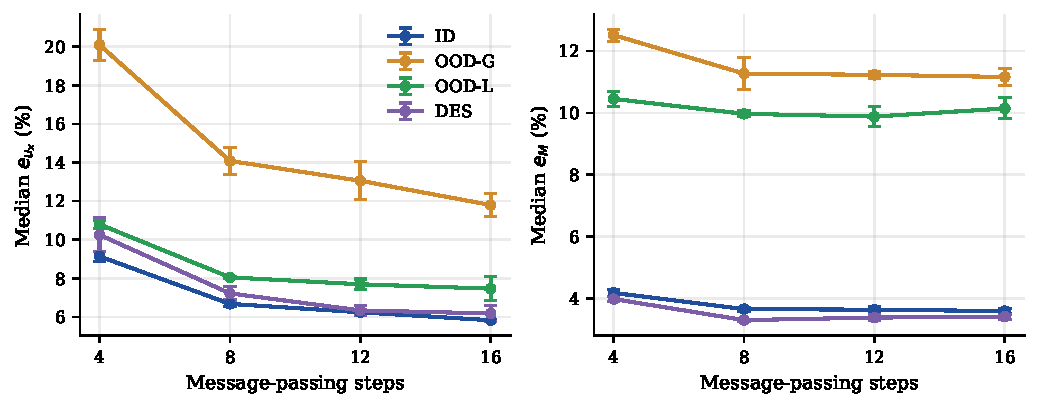
\includegraphics[width=\textwidth]{fig_depth.pdf}
\caption{Effect of the number of message-passing steps on the median displacement (left) and moment (right) errors of single networks (mean $\pm$ standard deviation over three seeds).}\label{fig:depth}
\end{figure}

\subsection{Equilibrium and the projection layer}\label{sec:eqresults}
Without the projection, every model produces member forces that are not in equilibrium with the applied loads (Fig.~\ref{fig:equilibrium}). The median out-of-balance force is 4\% of the load vector for the raw graph ensemble and 7--43\% for the tabular baselines on in-distribution frames, rising to 16\% and 18--120\% for unseen geometries. After projection (Eq.~\ref{eq:projection}) the residual is below $10^{-12}$ for every frame and every model, so the support reactions balance the loads and every nodal free body is in equilibrium.

\begin{figure}[t]
\centering
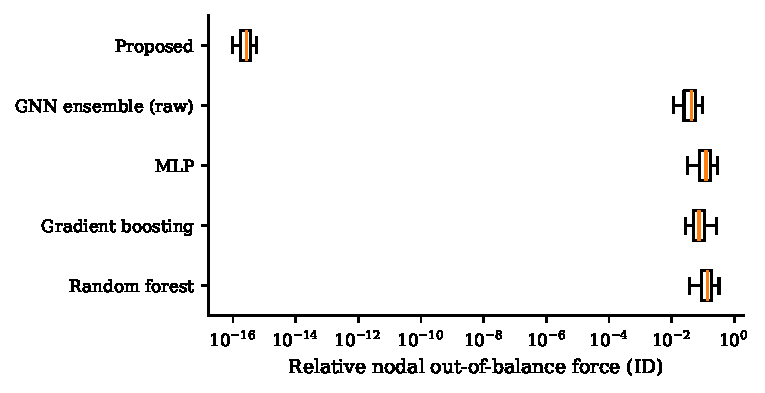
\includegraphics[width=0.75\textwidth]{fig_equilibrium.pdf}
\caption{Relative nodal out-of-balance force of the predicted member forces on the in-distribution test set (box: quartiles; whiskers: 5th--95th percentiles). Only the projected surrogate is statically admissible.}\label{fig:equilibrium}
\end{figure}

The metric of the projection matters. With the variance-weighted metric the axial-force error decreases by a factor of 2--4.7 (1.8\%$\to$0.6\% ID, 5.3\%$\to$1.5\% OOD-G, 3.5\%$\to$1.6\% OOD-L, 1.4\%$\to$0.3\% DES; Table~\ref{tab:compat}), the support-reaction errors by a factor of 2--3.5, and the moment errors decrease modestly (Section~\ref{sec:stats}). With the Euclidean metric the projection degrades the moments (2.5\%$\to$4.0\% ID, 8.3\%$\to$12.6\% OOD-G) while still improving the axial forces. This is consistent with Proposition~\ref{prop:projection}: the error can only decrease in the metric of the projection, and the Euclidean metric on dimensionless forces lets the correction flow into the moments, whose uncertainty it ignores.

\begin{table}[t]
\centering
\caption{Effect of the Euclidean equilibrium projection on the tabular baselines: median moment error $e_M$ and axial-force error $e_N$ (\%) before $\to$ after projection.}\label{tab:projbase}
\footnotesize
\setlength{\tabcolsep}{3pt}
\begin{adjustbox}{max width=\textwidth}
\begin{tabular}{lrrrrrrrr}
\toprule
& \multicolumn{2}{c}{ID} & \multicolumn{2}{c}{OOD-G} & \multicolumn{2}{c}{OOD-L} & \multicolumn{2}{c}{DES}\\
\cmidrule(lr){2-3}\cmidrule(lr){4-5}\cmidrule(lr){6-7}\cmidrule(lr){8-9}
Model & $e_M$ & $e_N$ & $e_M$ & $e_N$ & $e_M$ & $e_N$ & $e_M$ & $e_N$\\
\midrule
\inputtable{tables/tab_proj_baselines.tex}
\bottomrule
\end{tabular}
\end{adjustbox}
\end{table}

Because the layer is model-agnostic, it was also applied to the tabular baselines (Table~\ref{tab:projbase}), which provide no per-output variance, so the Euclidean metric is used. The axial-force errors decrease for every baseline and test set. The moment errors decrease for gradient boosting and for the MLP on most sets, but increase for the linear ridge model and the random forest; in the conventional GNN, whose Euclidean metric acts on physical forces, the projection reduces the moment errors (5.4\%$\to$4.4\% ID, 16.9\%$\to$12.7\% OOD-G), whereas for the dimensionless single networks it increases them (Table~\ref{tab:grapheq}). The projection therefore always delivers admissible forces and always improves the axial forces, while its effect on the moments depends on whether the metric reflects where the prediction errors actually are, which is what the ensemble variance provides.

\subsection{Displacement--force compatibility}\label{sec:compatresults}

\begin{table}[t]
\centering
\caption{Equilibrium and compatibility of the force fields of the proposed ensemble (ensemble 0): medians over the test frames (\%, residuals as fractions). $r_\mathrm{compat}$ and $r_{\mathrm{compat},M}$: Eq.~\eqref{eq:compat}; eq.\ res.: relative nodal out-of-balance force. The displacements are the same in all rows.}\label{tab:compat}
\footnotesize
\begin{adjustbox}{max width=\textwidth}
\begin{tabular}{lrrrrrr}
\toprule
Force field & $e_M$ & $e_N$ & $e_V$ & Eq.\ res. & $r_\mathrm{compat}$ & $r_{\mathrm{compat},M}$ \\
\midrule
\inputtable{tables/tab_compat.tex}
\bottomrule
\end{tabular}
\end{adjustbox}
\end{table}

Table~\ref{tab:compat} answers the question whether the projection makes the force field more or less compatible with the predicted displacements. The forces implied by the predicted displacements differ substantially from the predicted forces: the median compatibility residual of the raw ensemble is 47\% on the ID set and 87\% on unseen geometries. Most of this comes from the axial forces, because a displacement error of a few per cent, multiplied by the large axial stiffness $EA/L$, produces axial forces that are far from the true ones; restricted to the end moments the residual is 11\% (ID), 40\% (OOD-G), 18\% (OOD-L) and 4\% (DES). The equilibrium projection hardly changes these numbers. With the variance-weighted metric, $r_{\mathrm{compat},M}$ increases in 68\%, 67\%, 74\% and 69\% of the ID, OOD-G, OOD-L and DES frames, but only by a median factor of 1.01--1.04; with the Euclidean metric the increase is larger (median factor 1.03--1.34) and affects 82--93\% of the frames. The projection therefore slightly increases the incompatibility, as expected for a correction that acts on the forces alone, and the size of the increase follows the size of the force correction.

Recovering the forces from the predicted displacements, as in displacement-based surrogates~\cite{leng2026mcgnn}, gives zero compatibility residual by construction, but much less accurate forces and large equilibrium violations: the median moment error rises from 2.4\% to 11.2\% (ID) and from 7.5\% to 44.2\% (OOD-G), the axial-force errors reach 53\% and 183\%, and the out-of-balance force exceeds the applied load (median residual 1.7 and 9.8). Member forces are second derivatives of the displacement field, so the differentiation amplifies the displacement errors. In this setting, predicting the forces directly and imposing equilibrium is far more accurate than imposing compatibility, which is why the proposed workflow enforces the former and only measures the latter. A field that satisfies both is the FE solution. Using the predicted displacements as the starting point of a Jacobi-preconditioned conjugate-gradient solve of the full stiffness equations did not reduce the number of iterations to a relative residual of $10^{-8}$ (median 27 iterations for ID frames with and without the warm start; 72 for OOD-G), because the initial residual is dominated by the stiff axial DOFs: at the median it is 1.4 times (ID) and 12 times (OOD-G) the norm of the load vector, i.e.\ larger than the residual of a zero initial guess. A compatibility-aware correction that would help in practice would have to treat the axial and flexural parts separately and is left for future work.


\subsection{Sensitivity of the projection to the variance floor}\label{sec:sensitivity}

\begin{table}[t]
\centering
\caption{Sensitivity of the variance-weighted projection to the regularisation of $\boldsymbol{\Sigma}$ (ensemble 0): median moment error $e_M$ (\%) and largest condition number of $\mathbf{C}\boldsymbol{\Sigma}\mathbf{C}^{\mathsf T}$ over the frames of each set.}\label{tab:sensitivity}
\footnotesize
\begin{adjustbox}{max width=\textwidth}
\begin{tabular}{lrrrrrrrr}
\toprule
& \multicolumn{2}{c}{ID} & \multicolumn{2}{c}{OOD-G} & \multicolumn{2}{c}{OOD-L} & \multicolumn{2}{c}{DES}\\
\cmidrule(lr){2-3}\cmidrule(lr){4-5}\cmidrule(lr){6-7}\cmidrule(lr){8-9}
$\boldsymbol{\Sigma}$ & $e_M$ & $\kappa_{\max}$ & $e_M$ & $\kappa_{\max}$ & $e_M$ & $\kappa_{\max}$ & $e_M$ & $\kappa_{\max}$ \\
\midrule
\inputtable{tables/tab_sensitivity.tex}
\bottomrule
\end{tabular}
\end{adjustbox}
\end{table}

Table~\ref{tab:sensitivity} varies the floor of the variance-weighted metric. For floors between $10^{-8}\bar\sigma^2$ and $10^{-4}\bar\sigma^2$, and for the additive form of Eq.~\eqref{eq:sigmareg}, the median moment errors are identical to two decimals on every set (2.36, 7.51, 8.73 and 2.00\%), so the results do not depend on $\varepsilon$ in this range. A floor of $10^{-2}\bar\sigma^2$ changes them by at most 0.12 percentage points, while a floor equal to the mean variance, which makes the metric nearly uniform, moves the errors most of the way towards the Euclidean projection (3.9\% ID, 11.5\% OOD-G). The largest condition number of $\mathbf{C}\boldsymbol{\Sigma}\mathbf{C}^{\mathsf T}$ over all 2{,}100 test frames is $3.6\times10^{5}$ (median $4\times10^{3}$ on ID frames, $3.5\times10^{4}$ on OOD-G frames), which is harmless for the direct LU solve in double precision: the projected fields satisfy equilibrium to a relative residual below $10^{-12}$ in every frame.


\subsection{Uncertainty, domain check and FE referral}\label{sec:uqresults}\label{sec:triage}

\begin{table}[t]
\centering
\caption{Quality of the frame-level uncertainty indicators (ensemble 0, variance-weighted projection). $\rho_s$: Spearman rank correlation with the true moment error $e_M$; coverage: fraction of end moments within the ensemble mean $\pm2\sigma$; ``$>$10\%'': fraction of frames with $e_M>10\%$; recall: share of those frames among the 20\% with the largest spread; p95: 95th percentile of $e_M$ over all frames and over the 80\% with the smallest spread.}\label{tab:uq}
\footnotesize
\begin{adjustbox}{max width=\textwidth}
\begin{tabular}{lrrrrrrr}
\toprule
Set & $\rho_s$ (spread) & $\rho_s$ (eq.\ residual) & Coverage (\%) & $>$10\% (\%) & Recall (\%) & p95 all (\%) & p95, 80\% kept (\%)\\
\midrule
\inputtable{tables/tab_uq.tex}
\bottomrule
\end{tabular}
\end{adjustbox}
\end{table}

\begin{figure}[p]
\centering
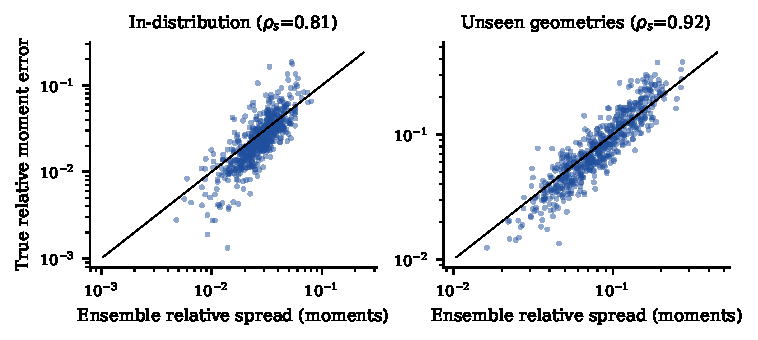
\includegraphics[width=\textwidth]{fig_uq_scatter.pdf}
\caption{Frame-level ensemble spread of the end moments $s$ (Eq.~\ref{eq:score}) against the true relative moment error for the four test sets. Black line: $e_M=s$; red dashed line: split-conformal bound $\hat a s$ calibrated on the validation frames.}\label{fig:uqscatter}
\end{figure}

The ensemble spread ranks the frames by their actual error well on in-distribution frames, on unseen geometries and on the design-driven frames (Spearman $\rho_s=0.81$, $0.92$ and $0.75$; Table~\ref{tab:uq} and Fig.~\ref{fig:uqscatter}), and the $\pm2\sigma$ intervals of the end moments contain 92\%, 92\% and 94\% of the PyNite values, close to the nominal 95\%. It is much weaker for unseen load patterns ($\rho_s=0.66$, coverage 67\%): the networks agree with each other on these frames while being wrong together, the known failure mode of ensembles under distribution shift~\cite{ovadia2019shift}. The label-free equilibrium residual of the raw prediction is a weaker indicator ($\rho_s=0.43$--$0.74$), which is why it is not used for referral.

\begin{table}[t]
\centering
\caption{Stage 1 of the referral rule: fraction of frames (\%) flagged as outside the training domain by the Mahalanobis distance of the frame descriptors, threshold at the 99th percentile of the validation frames.}\label{tab:ooddomain}
\footnotesize
\begin{tabular}{lrrrrr}
\toprule
Descriptors & Validation & ID & OOD-G & OOD-L & DES \\
\midrule
\inputtable{tables/tab_ood_domain.tex}
\bottomrule
\end{tabular}
\end{table}

The domain check (Table~\ref{tab:ooddomain}) flags 1.7\% of the ID test frames, close to the 1\% calibrated on the validation frames, and 79\% of the OOD-G and 75\% of the OOD-L frames. The two descriptor groups detect different shifts: the geometry descriptors flag 68\% of the unseen geometries but only 1.5\% of the unseen load patterns, and the load-pattern descriptors flag 67\% of the unseen load patterns but only 9\% of the unseen geometries. The load-pattern check therefore supplies exactly the information that the ensemble spread lacks. All 149 OOD-L frames that pass the check are frames whose random bay pattern happened to leave every bay fully loaded, so that only the lateral profile is new; the 129 OOD-G frames that pass are one step beyond the training range (45 have six storeys, 68 have five bays and at most five storeys). The check also flags 20\% of the design-driven frames, mainly because of their high gravity-to-lateral load ratio, their small roof share of the lateral load and their stiff material ($E$ at the upper end of the range), although the surrogate is accurate on all of them. The domain check is therefore conservative, which costs FE analyses but not accuracy.

\begin{table}[t]
\centering
\caption{Two-stage referral rule with thresholds fixed on the validation frames ($\hat a=1.41$ for $\alpha=0.1$). Referred: by the domain check, by the conformal bound $\hat a s>\tau$ and in total (\%). Coverage: share of in-domain frames with $e_M\le\hat a s$. Violation: share of accepted frames with $e_M>\tau$. p95: 95th percentile of $e_M$ over the accepted frames and over all frames (\%).}\label{tab:oodpolicy}
\footnotesize
\begin{adjustbox}{max width=\textwidth}
\begin{tabular}{llrrrrrrr}
\toprule
$\tau$ & Set & Domain & Bound & Total & Coverage & Violation & p95 accepted & p95 all \\
\midrule
\inputtable{tables/tab_ood_policy.tex}
\bottomrule
\end{tabular}
\end{adjustbox}
\end{table}

Table~\ref{tab:oodpolicy} evaluates the complete rule, whose two thresholds were fixed on the validation frames before the test sets were used. With a tolerance of $\tau=10\%$ on the relative moment error, the rule refers 2.2\% of the ID frames and accepts the rest with a violation rate of 1.4\% (frames whose true error exceeds 10\% although accepted). On unseen geometries it refers 86\% of the frames and the accepted 14\% have a 95th-percentile error of 7.7\% and a violation rate of 1.2\%, compared with a 95th percentile of 22.6\% and 35\% of frames above 10\% without referral. On unseen load patterns it refers 75\% and the accepted frames have a violation rate of 1.4\%. On the design-driven frames 20\% are referred by the domain check and none of the accepted frames exceeds 10\% (largest accepted error 4.8\%). With $\tau=5\%$ the violation rates are 3.5\% (ID), 17\% (OOD-G, 12 accepted frames), 5.4\% (OOD-L) and 0\% (DES), at the cost of referring 28\% of the ID frames. The conformal bound covers the true error in 90\% (ID), 94\% (OOD-G) and 99\% (DES) of the in-domain frames, matching the nominal 90\%, but only in 84\% of the in-domain OOD-L frames, so the coverage guarantee, which assumes exchangeability with the calibration frames, holds only approximately once the load pattern changes; the domain check is what keeps the accepted OOD-L frames safe. These numbers are the honest cost of the safety: the rule cannot make the surrogate accurate where it is not, but it makes the referral decision before the FE result is known and with thresholds that were not tuned on the test data.

\begin{figure}[p]
\centering
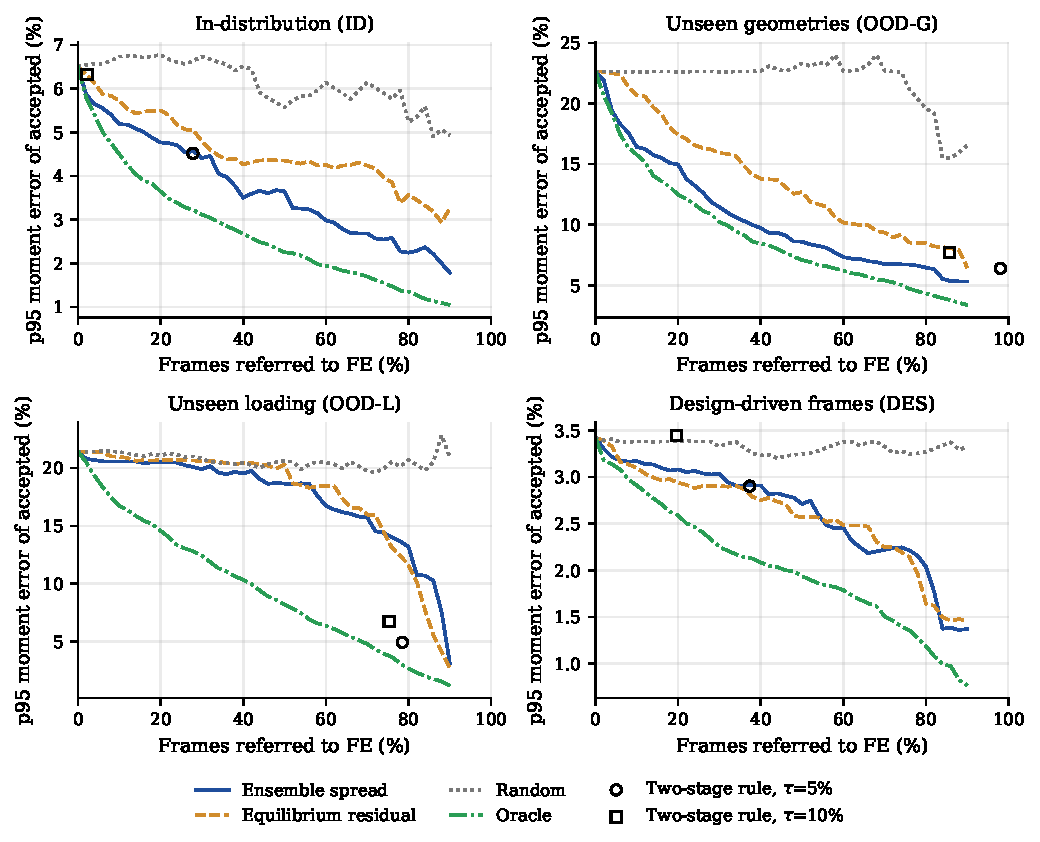
\includegraphics[width=\textwidth]{fig_triage.pdf}
\caption{Risk--coverage curves: 95th percentile of the moment error over the accepted predictions when the frames with the largest scores are referred to PyNite, for the ensemble spread, the equilibrium residual, random referral and an oracle ranking by the true error. Markers: operating points of the two-stage rule with validation-calibrated thresholds (Table~\ref{tab:oodpolicy}). The curves are computed on the test sets and serve only to describe the ranking quality.}\label{fig:triage}
\end{figure}

Figure~\ref{fig:triage} complements the rule with risk--coverage curves. On the ID set, referring the 20\% of frames with the largest spread lowers the 95th-percentile moment error from 6.5\% to 4.8\% and catches 78\% of the 1.5\% of frames with errors above 10\%. On unseen geometries it lowers the tail from 22.6\% to 15.0\%; on unseen load patterns the spread-based ranking is little better than random (21.4\%$\to$20.5\%), which is why the domain check is needed.


\subsection{Adaptive FE data generation}\label{sec:adaptive}
The adaptive study starts from 200 randomly chosen PyNite analyses and adds 200 per round up to 1{,}200, training a three-network ensemble (100 epochs) in every round; the whole study is repeated with two random seeds, and Fig.~\ref{fig:adaptive} shows the seed mean with the range of the two runs. Table~\ref{tab:adaptive} lists the errors at the final budget. Because these ensembles are smaller and trained on fewer frames for fewer epochs, their errors are higher than those of the main model in Table~\ref{tab:main}.

\begin{figure}[t]
\centering
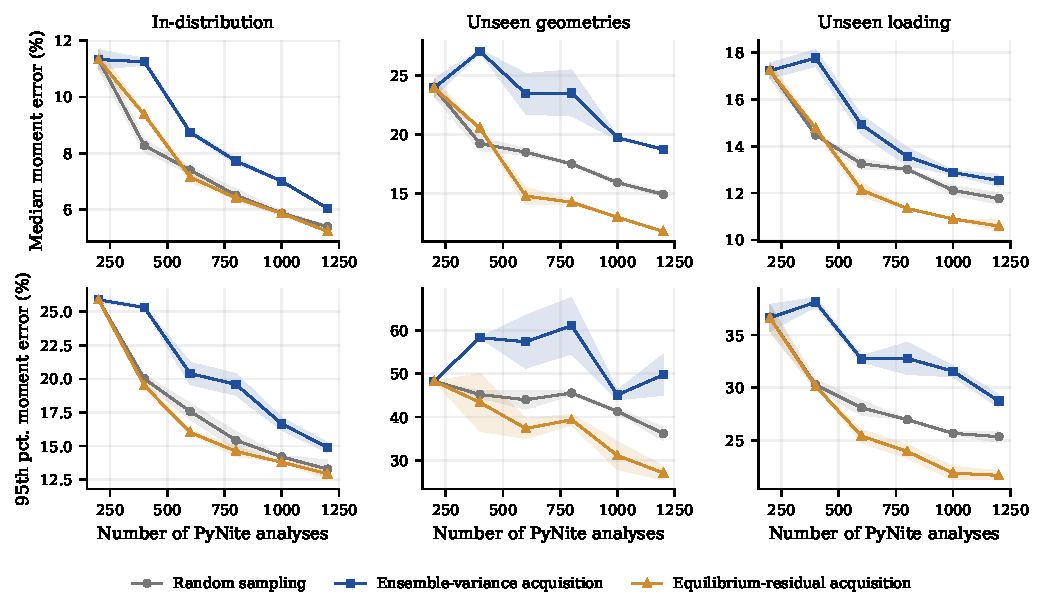
\includegraphics[width=\textwidth]{fig_adaptive.pdf}
\caption{Moment error (median, top; 95th percentile, bottom) versus the number of PyNite analyses used for training, for three acquisition rules. Lines: mean of two seeds; bands: range of the two seeds. Predictions include the variance-weighted projection.}\label{fig:adaptive}
\end{figure}

\begin{table}[t]
\centering
\caption{Errors (\%) after 1{,}200 PyNite analyses for each acquisition rule (mean of two seeds): median and 95th percentile of the moment error and median horizontal displacement error.}\label{tab:adaptive}
\scriptsize
\setlength{\tabcolsep}{3.5pt}
\begin{adjustbox}{max width=\textwidth}
\begin{tabular}{lrrrrrrrrr}
\toprule
& \multicolumn{3}{c}{In-distribution} & \multicolumn{3}{c}{Unseen geometries} & \multicolumn{3}{c}{Unseen loading}\\
\cmidrule(lr){2-4}\cmidrule(lr){5-7}\cmidrule(lr){8-10}
Acquisition & $e_M$ & $e_M$ (p95) & $e_{u_x}$ & $e_M$ & $e_M$ (p95) & $e_{u_x}$ & $e_M$ & $e_M$ (p95) & $e_{u_x}$\\
\midrule
\inputtable{tables/tab_adaptive.tex}
\bottomrule
\end{tabular}
\end{adjustbox}
\end{table}

Two findings stand out. First, selecting the frames with the largest ensemble variance is \emph{worse} than random sampling on all three test sets and for both seeds (median moment error 6.0\% vs.\ 5.4\% ID, 18.8\% vs.\ 14.9\% OOD-G at 1{,}200 analyses). Greedy top-$B$ selection by variance concentrates the budget on the most extreme corners of the design space, typically frames with very flexible members or unusual stiffness ratios, at the expense of coverage of the bulk of the distribution; a batch of 200 such frames is also highly redundant. Second, selecting the frames whose raw prediction is furthest from equilibrium is the best of the three rules for the member forces on every test set: at 1{,}200 analyses the median moment error is 5.2\% (random 5.4\%) on ID frames, 11.8\% (14.9\%) on unseen geometries and 10.6\% (11.8\%) on unseen loading, and the 95th percentile on unseen geometries falls from 36.2\% to 27.1\%. On unseen geometries the equilibrium-residual rule reaches the final error of random sampling after 600 analyses, i.e.\ with half the FE budget, and on unseen loading after 800. The gain is specific to forces: the displacement errors are similar to or slightly larger than with random sampling (Table~\ref{tab:adaptive}), which is expected, since the residual measures the admissibility of the forces only. With two seeds, the differences between the equilibrium-residual rule and random sampling on the ID set are within the seed-to-seed spread, whereas those on the unseen sets are consistent across both seeds.


\subsection{Computational cost}\label{sec:cost}
Timings were measured serially on the otherwise idle machine (Section~\ref{sec:protocol}), five times for 200 frames of each test set (Table~\ref{tab:timing}). Besides PyNite, two other solvers were timed on the same frames for both load cases: OpenSeesPy and the vectorised sparse direct-stiffness solver written for the verification (Section~\ref{sec:validation}), which represents an optimised minimal FE pipeline for this problem class. A PyNite analysis of one frame (two load cases, including model construction and result extraction) costs $33.6\pm1.6$\,ms for ID frames and $98.0\pm4.0$\,ms for the larger OOD-G frames. Evaluated in batches, the proposed surrogate costs 2.7\,ms (ID and OOD-L) and 7.0\,ms (OOD-G) per frame, including the Python feature construction (the largest part), the five-network ensemble and the projection (0.1--0.6\,ms), i.e.\ 12--14 times less than PyNite. For a single frame evaluated in isolation the overhead of the network framework dominates and the surrogate (20--87\,ms) is not faster than PyNite.

\begin{table}[t]
\centering
\caption{Wall-clock time per frame (ms; mean $\pm$ standard deviation over five repetitions of 200 frames, 4-core 2.1\,GHz CPU, networks evaluated with 4 threads): PyNite, OpenSeesPy and the sparse direct-stiffness solver (DSM) for both load cases; the proposed surrogate evaluated in batches and for one frame alone; batched speed-up relative to PyNite and to the DSM solver.}\label{tab:timing}
\footnotesize
\setlength{\tabcolsep}{3pt}
\begin{adjustbox}{max width=\textwidth}
\begin{tabular}{lrrrrrrr}
\toprule
Set & PyNite & OpenSeesPy & DSM & Surrogate (batched) & Surrogate (single) & vs PyNite & vs DSM\\
\midrule
\inputtable{tables/tab_timing.tex}
\bottomrule
\end{tabular}
\end{adjustbox}
\end{table}

The comparison with an optimised solver changes the picture. OpenSeesPy and the sparse direct-stiffness solver analyse a frame in 1.2--2.8\,ms, faster than the batched surrogate on every test set (speed-up of the surrogate over the DSM solver 0.34--0.65). Most of the cost of a PyNite analysis is the construction of the general three-dimensional model and the extraction of results through its object interface, not the solution of the linear system, which for frames with at most a few hundred DOFs takes well under a millisecond. Against PyNite, the batched surrogate pays back its one-off cost (about 41\,min of CPU time to train the five networks, while the 3{,}000 training analyses cost about 2\,min) only after roughly $8\times10^4$ ID frames without referral and $1.1\times10^5$ with 20\% of the frames referred to PyNite; against an optimised solver it never does. For first-order linear analysis of frames of this size the surrogate therefore offers no speed advantage over a well-implemented FE solver. Its value in this setting lies elsewhere: a differentiable, batched map from the frame parameters to the full response with a calibrated referral rule, which is useful for gradient-based design and for screening, and a template for analyses that are genuinely expensive (nonlinear, dynamic, or much larger models), which this paper does not test.

